\PassOptionsToPackage{svgnames}{xcolor}
\documentclass[11pt]{article}



\usepackage[margin=0.1in]{geometry}  
\usepackage{graphicx}             
\usepackage{amsmath}              
\usepackage{amsfonts}              
\usepackage{framed}               
\usepackage{amssymb}
\usepackage{array}
\usepackage{amsthm}
\usepackage{multirow}
\usepackage[nottoc]{tocbibind}
\usepackage{bm}
\usepackage{enumitem}
\usepackage{tikz}
\usepackage{pdfpages}

\usepackage{titlesec}
\titlespacing*{\section}{0pt}{0.5\baselineskip}{0.5\baselineskip}
\newcolumntype{C}[1]{>{\centering\let\newline\\\arraybackslash\hspace{0pt}}m{#1}}


  \newcommand\norm[1]{\left\lVert#1\right\rVert}
\setlength{\parindent}{0cm}
\setlength{\parskip}{0em}
\newcommand{\Lim}[1]{\raisebox{0.5ex}{\scalebox{0.8}{$\displaystyle \lim_{#1}\;$}}}
\newtheorem{definition}{Definition}[section]
\newtheorem{theorem}{Theorem}[section]
\newtheorem{notation}{Notation}[section]
\theoremstyle{definition}
\DeclareMathOperator{\arcsec}{arcsec}
\DeclareMathOperator{\arccot}{arccot}
\DeclareMathOperator{\arccsc}{arccsc}
\DeclareMathOperator{\spn}{Span}
\setcounter{tocdepth}{1}
\begin{document}

%\clearpage
\twocolumn
\section{Introduction to OS}
\subsection{Operating System Basic Concepts}
\begin{definition}[Operating System]
\normalfont An \textbf{operating system}(OS) is a program that acts as an intermediary between a \textbf{computer user} and the \textbf{computer hardware}.
\end{definition}
The evolution of OS is as below
\[
\text{No OS}\to\text{Batch OS}\to\text{Time-sharing OS}\to\text{Personal OS}
\]
\begin{definition}[No OS]
\normalfont There is no OS for the first computer where programmes \textit{directly} interact with hardware, and reprogramming is done through changing the \textbf{physical configuration} of the hardware.\\
\begin{figure}[h]
\centering
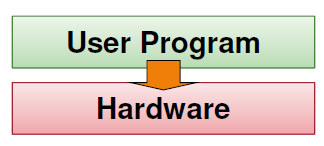
\includegraphics[width = 0.25\textwidth]{1_1.png}
\end{figure}
\textbf{Advantage}:
\begin{itemize}[itemsep=0pt]
  \item Minimal overhead
\end{itemize}
\textbf{Disadvantage}:
\begin{itemize}[itemsep=0pt]
  \item Programmes are not portable
  \item Utilisation of Computing resource is low
\end{itemize}
\end{definition}
\begin{definition}[Batch OS]
\normalfont Batch OS breaks down the workflow to Input, Compute and Output, which allows pipelining to occur.\\
Programmes can be \textit{submitted in batch} to be \textit{executed one at a time}. \\
\begin{figure}[h]
\centering
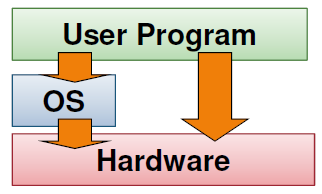
\includegraphics[width = 0.25\textwidth]{1_2.png}
\end{figure}
However, batch processing is still inefficient since the CPU will be idle when I/O. One solution is \textbf{multiprogramming}, where multiple jobs are loaded and other jobs are to be ran when I/O needs to be done.
\end{definition}
\begin{definition}[Time-sharing OS]
\normalfont Time-sharing OS allows multiple users to interact with machine using terminals(\textbf{teletypes}). It provides user job scheduling which gives \textit{illusion} of concurrency. \\
\begin{figure}[h]
\centering
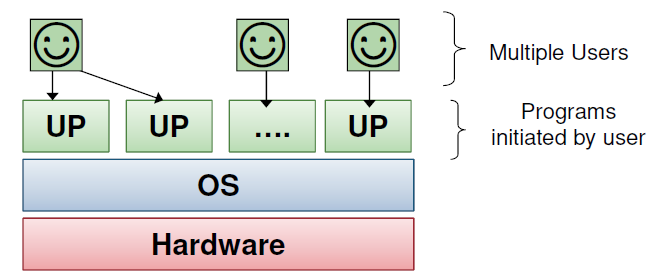
\includegraphics[width = 0.25\textwidth]{1_3.png}
\end{figure}
It provides CPU time, memory and storage management; essentially, it provides \textbf{virtualisation of hardware}, where each program executes as if it has all the resources to itself.
\end{definition}
\begin{definition}[Personal OS]
\normalfont Personal OS is dedicated to machine that dedicates to one user, which is not time shared.\\
There are several models:
\begin{enumerate}
  \item Windows Model:
  \begin{itemize}[itemsep=0pt]
    \item Single user at a time but possibly more than 1 user can access
    \item dedicated machine
  \end{itemize}
  \item Unix Model:
  \begin{itemize}[itemsep=0pt]
    \item One user at the workstation but others can access remotely
    \item General time sharing model
  \end{itemize}
\end{enumerate}
\end{definition}
\subsection{Motivation of OS}
There are three main motivations:
\begin{enumerate}
  \item Abstraction over the hardware, which has
  \begin{itemize}[itemsep=0pt]
    \item \textit{Different} capacity
    \item \textit{Different} capability, but
    \item Well-defined and \textit{common} functionality
  \end{itemize}
  so that low level details can be hidden and only high level functionality is presented. It provides efficiency and portability.
  \item Resource Allocator, which 
  \begin{itemize}[itemsep=0pt]
    \item Manages all resources such as CPU, Memory, I/O devices
    \item Arbitrate potentially conflicting requests, for efficient and fair resource use
  \end{itemize}
  \item Control Program, which controls execution of programmes so as to 
  \begin{itemize}[itemsep=0pt]
    \item Prevent errors and improper use of the computer, accidentally or maliciously
    \item Provide security and protection
  \end{itemize}
\end{enumerate}
\subsection{OS Structure}
Operating System structure needs to impart flexibility, robustness and maintainability. Generally, the high level view of OS is that
\begin{itemize}[itemsep=0pt]
  \item Operating system is essentially a \textbf{software}, which has the privilege to run in \textbf{kernel mode}, i.e., has complete access to all hardware resources
  \item Other software executes only in \textbf{user mode}, with limited access to hardware resources
\end{itemize}
\begin{figure}[h]
\centering
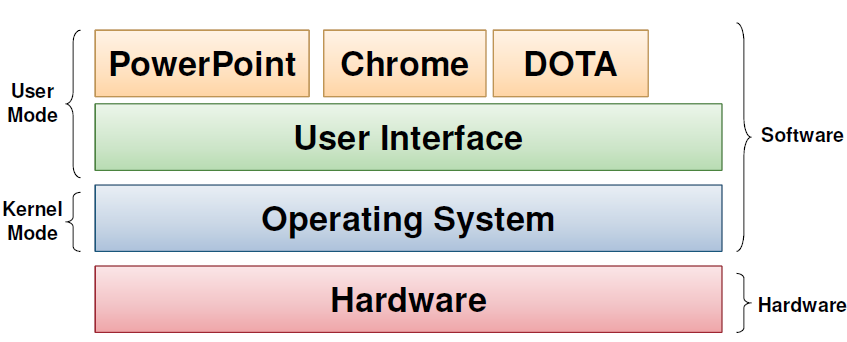
\includegraphics[width = 0.25\textwidth]{1_4.png}
\end{figure}
However, one must realise the user programme can interact with hardware through OS or else. Following diagram gives you an overview:
\begin{figure}[h]
\centering
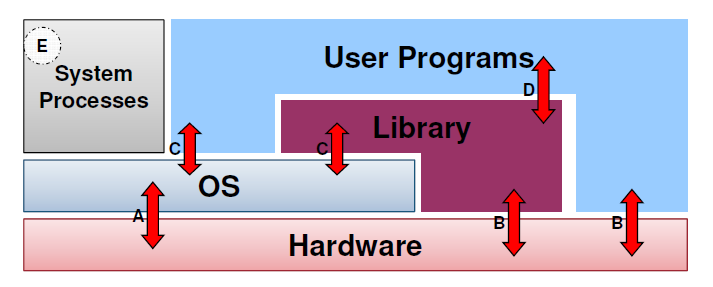
\includegraphics[width = 0.25\textwidth]{1_5.png}
\end{figure}
\begin{itemize}[itemsep=0pt]
  \item $A$: OS executing machine instructions
  \item $B$: normal machine instructions executed
  \item $C$: calling OS using \textbf{system call interface}, e.g. \texttt{fopen()}
  \item $D$: user program calls library code, e.g. \texttt{pow()}
  \item $E$: system processes, which provide \textit{high} level services, and is usually part of the OS
\end{itemize}

In terms of functionality, OS is known as the \textbf{kernel}, which is a programme providing special features like:
\begin{itemize}[itemsep=0pt]
  \item Deals with hardware issues
  \item Provides system call interface
  \item Special code for interrupt handlers, device drivers
\end{itemize}
However, kernel code has to be different than normal program as
\begin{itemize}[itemsep=0pt]
  \item No use of system call in kernel code
  \item Cannot use normal libraries
  \item There is no normal I/O
\end{itemize}
Currently, the common code organisation consists of
\begin{itemize}[itemsep=0pt]
  \item Machine independent high level language(HLL)
  \item Machine dependent HLL
  \item Machine dependent assembly code
\end{itemize}
In terms of implementation, there are few ways to structure an OS, most notably monolithic or microkernel.
\begin{definition}[Monolithic OS]
\normalfont Monolithic OS kernel has the defining characteristics of
\begin{itemize}[itemsep=0pt]
  \item One \textbf{big} special program, where various services and compopnents are integral part.
\end{itemize}
\begin{figure}[h]
\centering
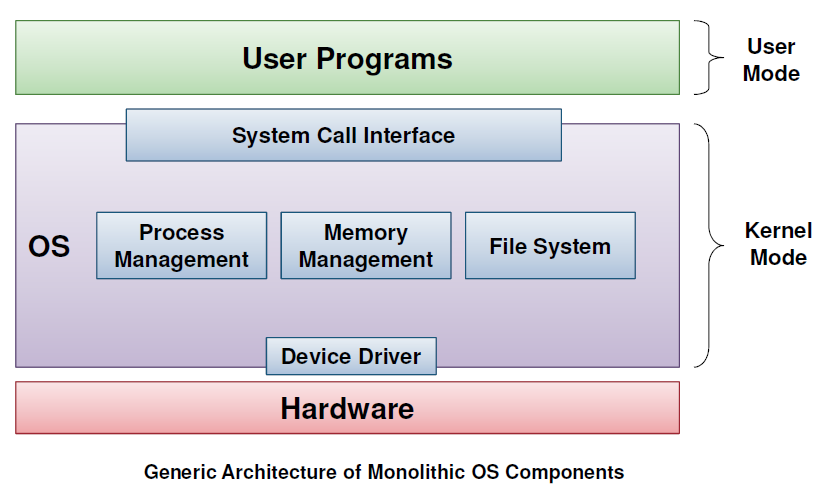
\includegraphics[width = 0.25\textwidth]{1_6.png}
\end{figure}
Monolithic kernel has the advantage of
\begin{itemize}[itemsep=0pt]
  \item Well understood
  \item Good performance
\end{itemize}
It has the disadvantage of
\begin{itemize}[itemsep=0pt]
  \item Highly coupled components
  \item Usually devolved into very complicated internal structure
\end{itemize}
\end{definition}
\begin{definition}[Microkernel OS]
\normalfont Microkernel OS kernel has the defining characteristics of 
\begin{itemize}[itemsep=0pt]
  \item Very small and clean
  \item Only provides basic and essential facilities:
  \begin{itemize}[itemsep=0pt]
    \item Inter-Process Communication(IPC)
    \item Address space management
    \item Thread management
    \item etc
  \end{itemize}
\end{itemize}
Higher level services like Process Management are
\begin{itemize}[itemsep=0pt]
  \item Built \textit{on top of} the basic facilities
  \item Run as server process \textbf{outside} of the OS
  \item Use IPC to communicate
\end{itemize}
\begin{figure}[h]
\centering
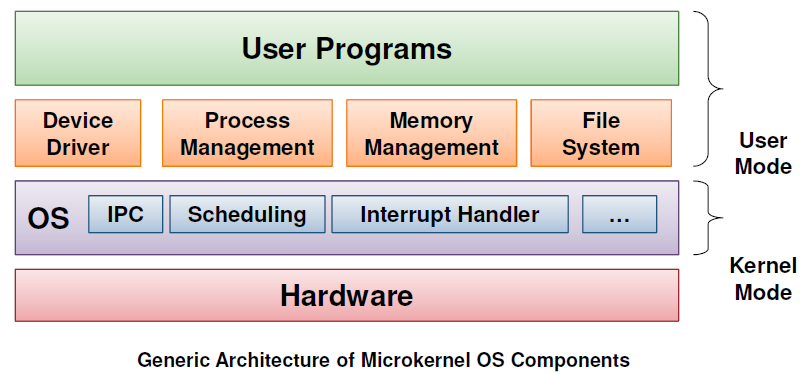
\includegraphics[width = 0.25\textwidth]{1_7.png}
\end{figure}
Microkernel OS has the advantage of
\begin{itemize}[itemsep=0pt]
  \item Kernel is generally more robust and more extendible
  \item Better isolation and protection between kernel and high level services
\end{itemize}
It has the disadvantage of
\begin{itemize}[itemsep=0pt]
  \item Lower performance
\end{itemize}
\end{definition}
Other OS structure include layered systems, client-server model etc.
\begin{definition}[Virtual Machine]
\normalfont Virtual Machine, or \textbf{hypervisor} is a software emulation(virtualisation) of hardware.
\end{definition}
Normal(primitive) operating systems can then run on top of the virtual machine.\\
There are two type of hypervisor:
\begin{figure}[h]
\centering
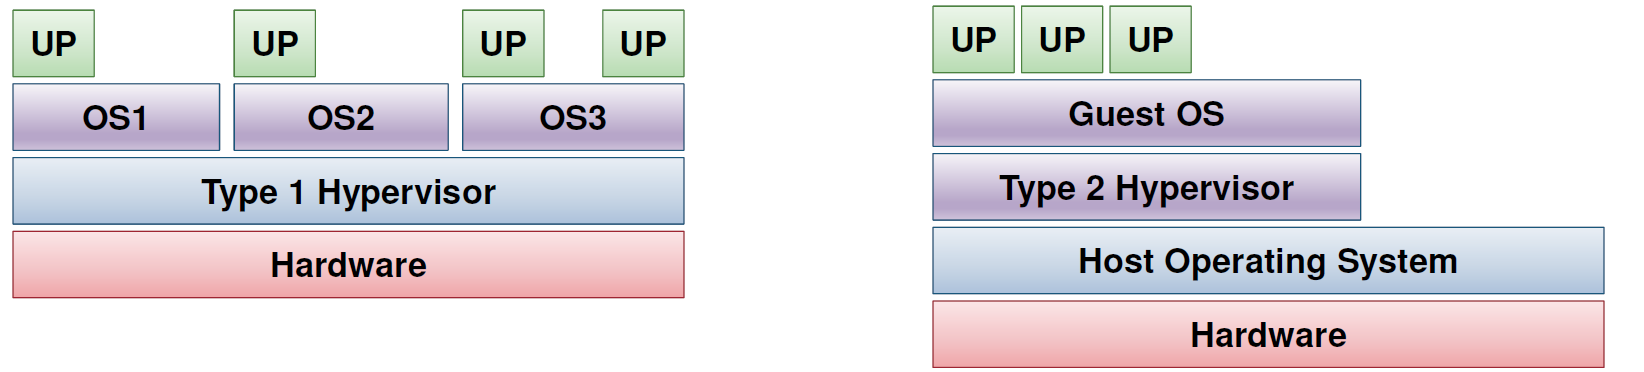
\includegraphics[width = 0.25\textwidth]{1_8.png}
\caption{Type 1 Hypervisor(left) and Type 2 Hypervisor(right)}
\end{figure}
\begin{itemize}[itemsep=0pt]
  \item Type 1: provides individual virtual machines to guest OSes
  \item Type 2: runs in host OS and only guest OS runs in Virtual Machine
\end{itemize}
%\clearpage
\section{Process Abstraction}
As the OS, to be able to switch from running program $A$ to $B$ requires
\begin{enumerate}
  \item Information regarding the execution of program $A$ to be stored
  \item Program $A$'s information is replaced with te information required to run $B$
\end{enumerate}
\begin{definition}[Process]
\normalfont \textbf{Process}/task/job is a dynamic abstraction for executing program, where information required to describe a running program is contained. The information includes three components:
\begin{itemize}[itemsep=0pt]
  \item Memory context
  \item Hardware context
  \item OS context
\end{itemize}
\end{definition}
\subsection{Memory Context}
From \texttt{CS2100}, we know that memory contains a 
\begin{itemize}[itemsep=0pt]
  \item \textbf{Text} section, to store instructions
  \item \textbf{Data} section, to store global variables
\end{itemize}
However, these two sections are unable to handle function call.
\begin{definition}[Caller, Callee]
\normalfont When \texttt{f()} calls \texttt{g()}, \texttt{f()} is the \textbf{caller} whereas \texttt{g()} is the \textbf{callee}.
\end{definition}
To handle function call, we require a new section called \textbf{Stack}.
\begin{definition}[Stack]
\normalfont Stack is used to store information about function invocation. The information of a function invocation is described by a \textbf{stack frame}.\\
Since stack can be of variable size, the top of the stack region is logically indicated by \textbf{stack pointer}. Stack pointer usually is stored in a specialised register in the CPU.
\begin{figure}[h]
\centering
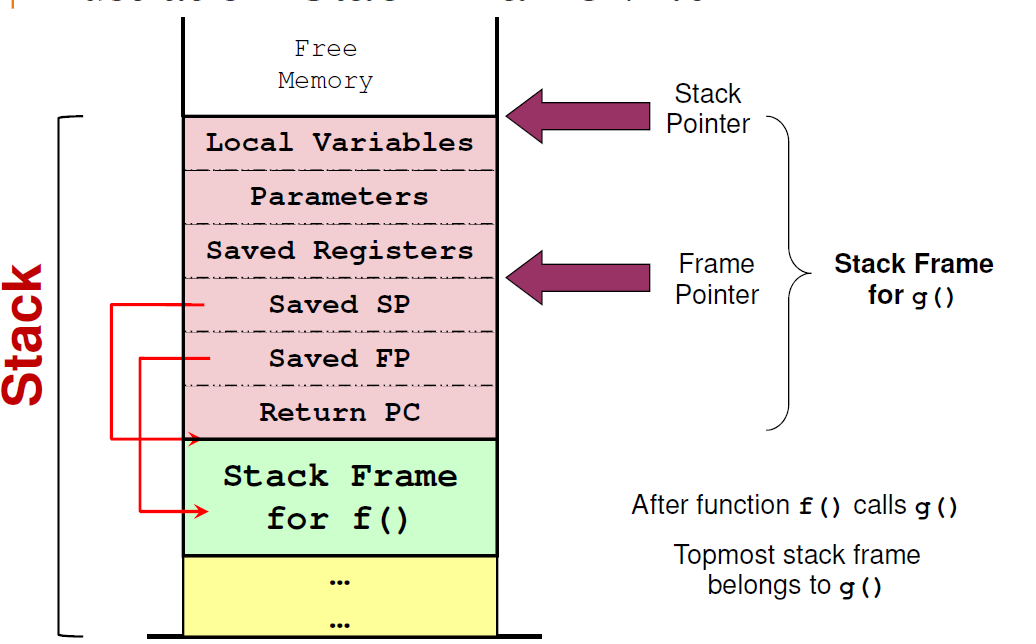
\includegraphics[width=0.25\textwidth]{2_1.png}
\end{figure}
Usually, a stack farme contains the following items
\begin{itemize}[itemsep=0pt]
  \item Local variables
  \item Function parameters
  \item Saved Registers
  \item Saved Stack Pointer
  \item Saved Frame Pointer
  \item Return Programme Counter(PC)
\end{itemize}
\end{definition}
\begin{definition}[Frame Pointer]
\normalfont Stack pointer can move during function execution. For example, the stack pointer can shift during a control statement \texttt{if}.\\
To facilitate the access of various stack frame items, a \textbf{frame pointer} can be used, which points to a \textbf{fixed location} in a stack frame. Other items can be accessed as a displacement from the frame pointer.
\end{definition}
\begin{theorem}[Stack Frame Setup/Teardown]
\normalfont On executing function call,
\begin{enumerate}
  \item \textbf{Caller}: Pass arguments with registers and/or stack
  \item \textbf{Caller}: Save Return PC on stack
  \item \textbf{Transfer control from caller to callee}
  \item \textbf{Callee}: Save registers used by callee. Save old FP, SP.
  \item \textbf{Callee}: Allocate space for local variables of callee on stack
  \item \textbf{Callee}: Adjust SP to point to new stack top
\end{enumerate}
On returning from function call:
\begin{enumerate}
  \item \textbf{Callee}: Restore saved registers, FP, SP
  \item \textbf{Transfer control from callee to caller using saved PC}
  \item \textbf{Caller}: Continues execution in caller
\end{enumerate}
\end{theorem}
\textbf{Remark}: There is no universal way of doing function call. The above is just a example.
\begin{definition}[Heap Memory Region]
\normalfont Heap Memory Region is a memory region that supports \textbf{dynamically allocated memory}, which is acquisition of memory space during \textbf{execution time}.
\end{definition}
Heap memory is trickier to manage due to its nature:
\begin{itemize}[itemsep=0pt]
  \item Variable Size
  \item Variable Allocation/Deallocation Timing
\end{itemize}
Its nature will create scenario where heap memory are allocated and deallocated in a way that creates holes in memory.\\

The actual memory context contains the four regions described above, namely text, data, heap and stack.
\begin{figure}[h]
\centering
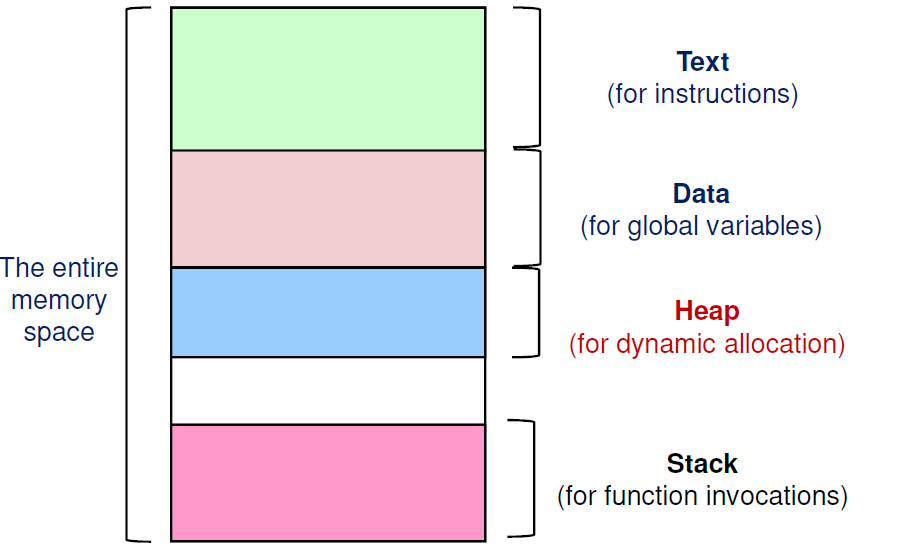
\includegraphics[width=0.25\textwidth]{2_2.png}
\end{figure}
\subsection{Hardware Context}
In correspondence to the memory context, the hardware context contains
\begin{itemize}[itemsep=0pt]
  \item General Purpose Registers
  \item Program Counter
  \item Stack Pointer
  \item Stack Frame Pointer
\end{itemize}
\subsection{OS Context}
\begin{definition}[Process ID]
\normalfont Process ID is to distinguish processes from each other, and it is unique among processes.
\end{definition}
Apart from Process ID, we also need a process state, to describe the state of the process, e.g. running or not running.
\begin{definition}[Generic 5-state Process Model]
\begin{figure}[h]
\centering
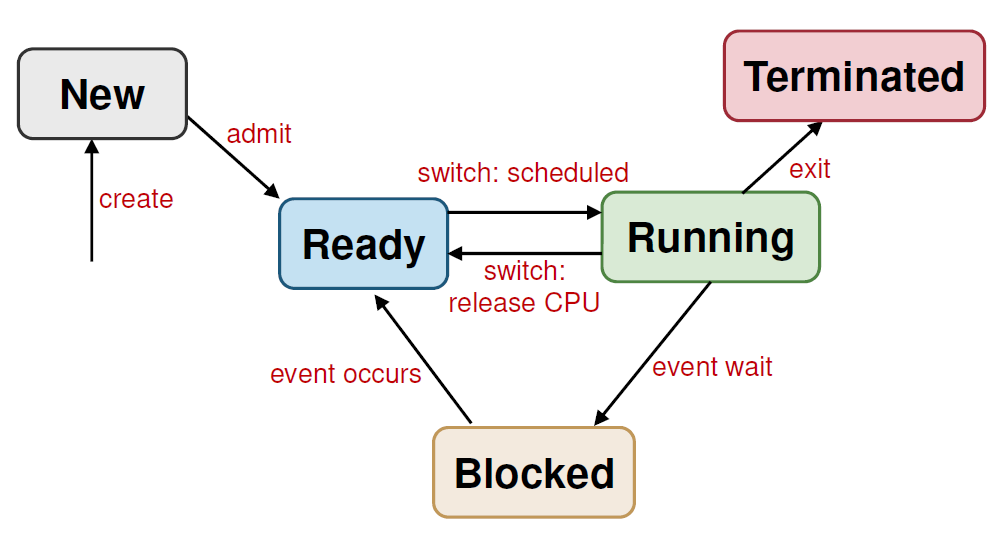
\includegraphics[width=0.25\textwidth]{2_3.png}
\end{figure}
\normalfont The Generic 5-state Process Model contains 5 states:
\begin{enumerate}
  \item New
  \begin{itemize}[itemsep=0pt]
    \item New process created
    \item May still be under initialisation, therefore \textit{not yet} ready
  \end{itemize}
  \item Ready
  \begin{itemize}[itemsep=0pt]
    \item Process is waiting to run
  \end{itemize}
  \item Running
  \begin{itemize}[itemsep=0pt]
    \item Process is being executed on CPU
  \end{itemize}
  \item Blocked
  \begin{itemize}[itemsep=0pt]
    \item Process waiting/sleeping for event
    \item Cannot execute until event is available
  \end{itemize}
  \item Terminated
  \begin{itemize}[itemsep=0pt]
    \item Process has finished execution, may require OS cleanup
  \end{itemize}
\end{enumerate}
There are also different state transitions,
\begin{enumerate}
  \item Create(NIL $\to$ New): new process is created
  \item Admit(New $\to$ Ready): process ready to be scheduled for running
  \item Switch(Ready $\to$ Running): process selected to run
  \item Switch(Running $\to$ Ready): process gives up CPU voluntarily or \textbf{pre-empted} by scheduler
  \item Event Wait(Running $\to$ Blocked): Process requests event/resource/service(system call, I/O, etc.) which is not available, or in progress
  \item Event Occurs(Blocked $\to$ Ready): Event occurs, which means process can continue
\end{enumerate}
\end{definition} 
In CS2106, we admit a simplified view on CPU: there is only 1 CPU, which means there is
\begin{itemize}[itemsep=0pt]
  \item $\leq 1$ process in running state
  \item conceptually 1 transition at a time
\end{itemize}
As there may be multiple processes ready for run, or awaiting resources, we use a queuing model to describe the 5-state transition.
\begin{figure}[h]
\centering
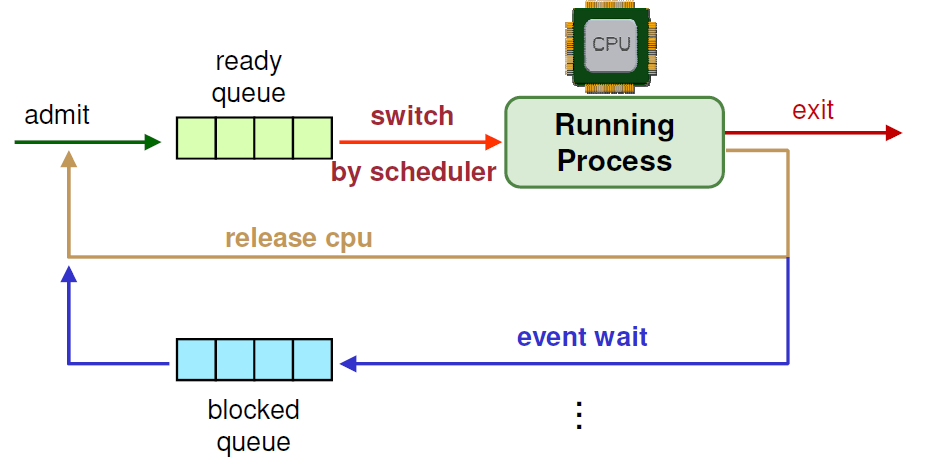
\includegraphics[width=0.25\textwidth]{2_4.png}
\end{figure}
Note, here the ready queue and the blocked queue should be viewed as \textbf{set}, not queue.\\

Up to this point, the OS context contains
\begin{itemize}[itemsep=0pt]
  \item Process ID,
  \item Process State
\end{itemize}
\subsection{Process Control Block}
The entire execution context for a process is stored in \textbf{Process Control Block}, maintained by the kernel. The process control block(PCB) contains memory, hardware and process context.\\
\begin{figure}[h]
\centering
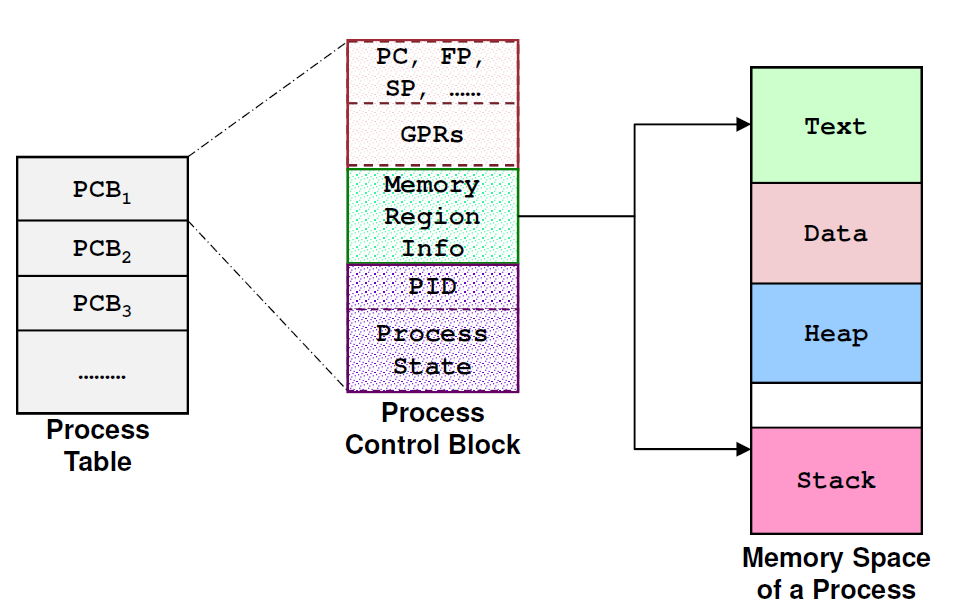
\includegraphics[width=0.25\textwidth]{2_5.png}
\end{figure}
 A process Table contains process control blocks of all processes.
\subsection{System Calls}
System calls are Application Program Interface(API) to OS, which provides ways of calling facilities/services in kernel.\\It is \textbf{not} the same as normal function call since it has to change from user mode to kernel mode.\\
Different OS will then have different APIs, for example:
\begin{itemize}[itemsep=0pt]
  \item UNIX variant: POSIX standard, which has small number($\approx 100$) of calls
  \item Windows family: Win API, which has $\approx 1000$ number of calls
\end{itemize}
In \texttt{C}, system calls can be invoked almost directly, but the function we call is not the actual system call, as we need to have a setup before the actual call. Therefore, the function we call can be
\begin{itemize}[itemsep=0pt]
  \item Function Wrapper, which is the same name and has the same parameters and the actual call, but handles the setup for caller. \\One example is \texttt{getpid()}.
  \item Function Adapter, which is a library function with less number of parameters and possibly more flexible parameter values.\\One example is \texttt{printf()}, which uses \texttt{write()} system call in its implementation.
\end{itemize}
\begin{theorem}[General System Call Mechanism]
\normalfont Generally, system call by user programme is handled in this manner:
\begin{enumerate}
  \item User program invokes the library call
  \item Library call, usually in assembly code, places the \textbf{system call number} is a designated location, e.g., a register.
  \item Library call executes a special instruction to switch from user mode to kernel mode. The special instruction is commonly known as \textbf{TRAP}. 
  \item Now, in kernel mode, the appropriate system call handler is determined, by using the system call number as an index. \\This step is usually handled by a \textbf{dispatcher}.
  \item System call handler is executed, carrying out the actual request.
  \item System call handler ended, and control is returned to the library call. \\We switch from kernel mode back to user mode.
  \item Library call return to the user program, via normal function return mechanism.
\end{enumerate}
\end{theorem}
\subsection{Exception and Interrupt}
\subsubsection{Exception}
Executing a \textbf{machine level instruction} can cause exception. For example, arithmetic error, or memory accessing errors are two common types of exceptions.\\
Exception is \textbf{synchronous}, in the sense that it occurs due to the program execution.\\
The effect of exception is 
\begin{itemize}[itemsep=0pt]
  \item Have to execute a \textbf{exception handler}. This exception handler is similar to a \textbf{forced function call}.
\end{itemize}
\subsubsection{Interrupt}
\textit{External} events can interrupt the execution of a program. The cause of interrupt is usually hardware related, for example \texttt{Ctrl + C}.\\
Interrupt, unlike exception, is therefore \textbf{asynchronous}, as it occurs independent of program execution.\\
The effect of interrupt is
\begin{itemize}[itemsep=0pt]
  \item Program execution is suspended, by executing an \textbf{interrupt handler}.
\end{itemize}
For the exception/interrupt handler, it is transferred control automatically to when an exception/interrupt occurs. Inside the handler, it performs the following routine
\begin{enumerate}
  \item Save Register/CPU state
  \item Perform the handler routine
  \item Restore Register/CPU
  \item Return from interrupt
\end{enumerate}
After the return from handler routine, program execution will resume, and the programme \textit{may} behave as if nothing happened.
%\clearpage
\section{Process Abstraction in UNIX}
\subsection{Identification}
A process in UNIX is uniquely identified by Process ID(PID), which is integer-valued.
\subsection{Information}
A process will keep track of the information of
\begin{itemize}[itemsep=0pt]
  \item \textbf{Proecss State}: Running, Sleeping, Stopped, Zombie
  \item \textbf{Parent PID}: PID of the parent process
  \item \textbf{Cumulative CPU time}: Total Amount of CPU time used so far
  \item etc
\end{itemize}
Unix command \texttt{ps} can extract the process information
\subsection{Process Creation}
\texttt{fork()} is the main way to create a new process. It returns
\begin{itemize}[itemsep=0pt]
  \item \texttt{PID} of the newly created process for parent process, or
  \item $0$ for child process
\end{itemize}
The behaviour of \texttt{fork()} is to create a new process called \textbf{child process}, which is a \textbf{duplicate} of the current executable image. The data in child is a \textbf{copy} of the parent, thus not shared. The \textit{only} difference between the parent and child process are
\begin{itemize}[itemsep=0pt]
\item Process ID(PID)
\item Parent ID(PPID)
\item \texttt{fork()} return value
\end{itemize}
Note, after \texttt{fork()}, both parent and child processes continue executing after \texttt{fork()}. If we want to make parent and child processes to behave differently, we can leverage on the \texttt{fork()} return value.
\subsection{Executing New Programe/Image}
\texttt{fork()} is not useful if you want to execute the original process and another process which is different from the original. Suppose the another process' code is provided as a new executable, then we can use \texttt{exec()} system calls family.\\

Specifically, one can use \texttt{execl()} to \textbf{replace} current executing process image with a new one. This replacement will change 
\begin{itemize}[itemsep=0pt]
  \item Code
  \item Memory content
\end{itemize}
but PID and other information will still be \textit{intact}.\\
\texttt{execl} takes the form of \texttt{execl const char *path, const char *arg0,...,const char *argN, NULL)}, where
\begin{itemize}[itemsep=0pt]
  \item \texttt{path} is the location of the executable
  \item \texttt{arg0} is the executable name
  \item \texttt{arg1} to \texttt{argN} are vararg command line arguments, corresponding to \texttt{argv[1]} to \texttt{argv[n]}.
  \item The last \texttt{NULL} is used to terminate the vararg array.
\end{itemize}
Therefore, we can combine \texttt{fork()} with \texttt{exec()} to
\begin{itemize}[itemsep=0pt]
  \item Spawn off a child process via \texttt{fork()}, which is replaced to the actual task process by invoking \texttt{exec()}.
  \item Parent process remains intact, which can continue to execute.
\end{itemize}
In fact, this way of invoking new processes is common across UNIX. Therefore, to start off, we need a special initial process, namely the \texttt{init} process, which is created in kernel at boot up time with a PID 1. The \texttt{init} process watches for other processes and respawns where needed. Other processes are created by invoking \texttt{fork()} on \texttt{init} or child of \texttt{init}. 
\subsection{Process Termination}
To end execution of process, we can use \texttt{exit(status)}. The status will be returned to the parent process, by which this child process is created.\\
The UNIX convention is to \texttt{exit} with a status $0$ if the termination is normal, and non-zero if the execution is problematic.\\
\textbf{Remark}: This function itself does not return.\\
When \texttt{exit(status)} is executed, \textit{most} system resources used by process are released. However, some basic process resources are \textbf{not releasable}. This includes
\begin{itemize}[itemsep=0pt]
\item PID and status, which is required for parent-children synchronisation
\item Process accounting information, e.g., CPU time\
\item Also, process table entry \textit{may be} still needed
\end{itemize}   
As most programs do not have explicit \texttt{exit()} call, return from main function will implicitly calls \texttt{exit()}, and as a result, open files will get flushed automatically, since file descriptors will be released.
\subsection{Parent/Child Synchronisation}
Parent process can wait for child process to terminate, by invoking \texttt{wait(*status)}. This call of \texttt{wait(*status)} will return the PID of the terminated child process. Also, the address where the \texttt{status} pointer points to will be populated with the exit status of the terminated child process.\
The behaviour of \texttt{wait()} is as follows
\begin{itemize}[itemsep=0pt]
  \item \texttt{wait()} is blocking: parent process is blocked until at least one child terminates
  \item The call cleans up \textbf{remainder} of the child system resources, which includes
  \begin{itemize}[itemsep=0pt]
    \item Those not removed on \texttt{exit()}, and also
    \item Kills zombie process
  \end{itemize}
\end{itemize}
Other variant of \texttt{wait()} includes
\begin{itemize}[itemsep=0pt]
  \item \texttt{waitpid()}, which waits for a specific child proecss
  \item \texttt{waitid()}, which waits for any child process to \textbf{change status}
\end{itemize}
Therefore, we can summarise the process interaction in UNIX as follows:
\begin{figure}[h]
\centering
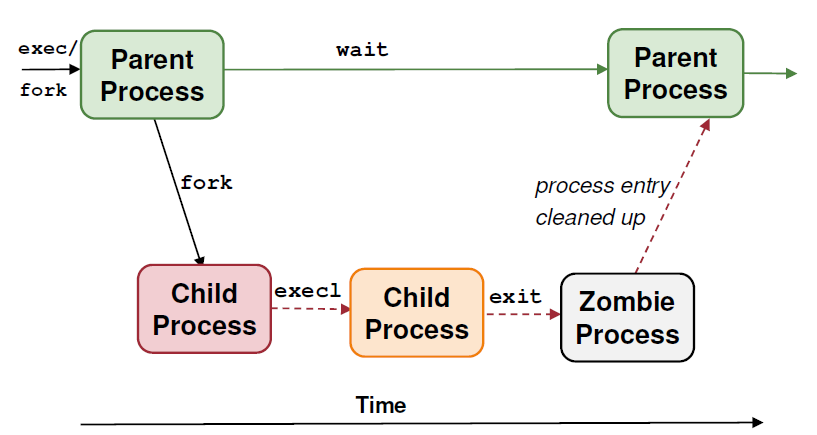
\includegraphics[width=0.25\textwidth]{3_1.png}
\end{figure}
Therefore, one point to note is that, suppose the parent does not \texttt{wait}, the zombie process cannot be cleaned up by the parent. Therefore, to handle this scenario, there are two cases to consider:
\begin{itemize}[itemsep=0pt]
  \item[Case 1] Parent process terminates before child process:
  \begin{itemize}[itemsep=0pt]
    \item \texttt{init} process becomes "pseudo" parent of child processes
    \item Child termination sends signal to \texttt{init}, which utilises \texttt{wait} to cleanup.
  \end{itemize}
  \item[Case 2] Child process terminates before parent, but parent did not call \texttt{wait}
  \begin{itemize}[itemsep=0pt]
    \item Child process becomes zombie, which can fill up the process table
    \item Therefore, we need to reboot to clear the table on older UNIX implementations.
  \end{itemize}
\end{itemize}
%\clearpage
\section{Process Scheduling}
We hope to achieve parallelism between processes, and therefore, \textbf{timeslicing} is used to share CPU time between processes, with OS occupying CPU between different processes to do the context switch.\\
In this sense, CPU is a \textbf{scheduler} deployed with certain \textbf{scheduling algorithm}. The specific scheduling algorithm will be influenced by \textbf{process behaviour and process environment}, but it should achieve a few common criteria to ensure its performance.\\

There are two main type of process behaviour:
\begin{itemize}[itemsep=0pt]
  \item \textbf{CPU-Activity}, such as computation. \\\textbf{Compute bound} process spend majority of time here.
  \item \textbf{IO-Activity}, such as printing to screen.\\\textbf{IO Bound} process spend majority of time here.
\end{itemize}
There are three main type of processing environment, namely
\begin{enumerate}
  \item \textbf{Batch Processing}, where there is \textit{no} interaction required and there is \textit{no} need to be responsive.
  \item \textbf{Interactive}, where there are active user(s) interacting with system, therefore process should be responsive and consistent in response time
  \item \textbf{Real time processing}, where there are deadline to meet.
\end{enumerate}
In this course, we are only concerned about (1) and (2).\\

There are two criteria that is applicable for \textbf{all processing environments}:
\begin{itemize}[itemsep=0pt]
  \item Fairness
  \begin{itemize}[itemsep=0pt]
    \item Each process, or each user should get a fair share of CPU time
    \item There should not be starvation for certain processes
  \end{itemize}
  \item Balance
  \begin{itemize}[itemsep=0pt]
    \item All parts of the computing systems should be utilised
  \end{itemize}
\end{itemize}
There are two types of scheduling policies, defined by when scheduling is triggered.
\begin{itemize}[itemsep=0pt]
  \item \textbf{Non-preemptive}: where a process stayed scheduled (in running state) until it blocks or give up CPU voluntarily
  \item \textbf{Preemptive}: where a process is given a fixed time quota to run. Process can either give up early or give up due to blocking, or be suspended by OS to give another process CPU time, if available.
\end{itemize}

The step by step scheduling algorithm is as below:
\begin{enumerate}
  \item Scheduler is triggered.
  \item If context switch is nedded, save current running process' context and place it on blocked/ready queue
  \item Pick a suitable process $P$ to run based on scheduling algorithm
  \item Setup context for $P$
  \item Run $P$
\end{enumerate}
\subsection{Scheduling for Batch Processing}
Since there is no user interaction, we will try to optimise for the criteria below:
\begin{itemize}[itemsep=0pt]
  \item Minimise Turnaround time, which is calculated as finish time $-$ arrival time.
  \item Throughput, which is number of tasks finished per unit time
  \item CPU utilisation, which is percentage of time when CPU is working on a tak
\end{itemize}
\subsubsection{First Come First Served(FCFS)}
In \textbf{First Come First Served} scheduling, 
\begin{itemize}[itemsep=0pt]
  \item Tasks are stored on a First-In-First-Out (FIFO) queue based on arrival time
  \item Pick the first task in queue to run until:
  \begin{itemize}[itemsep=0pt]
    \item Task is done
    \item Task is blocked
  \end{itemize}
  \item Blocked task is removed from the FIFO queue, and is placed at the back of queue when it is ready again
\end{itemize}
This algorithm is good as it is guaranteed to have \textbf{no starvation}, since no process can jump queue.\\
This algorithm is not optimal as 
\begin{itemize}[itemsep=0pt]
  \item Simple reordering of jobs can reduce average waiting time
  \item The convoy effect on processes, in which a long-running process is followed by small processes, and the first long-running process will block every short processes at the back for CPU, IO etc if they require the same resource.
\end{itemize}
\subsubsection{Shortest Job First(SJF)}
In \textbf{shortest job first} scheduling, after any process is finished running, we select a task with smallest total CPU time.\\
It is a good algorithm since it \textit{minimises} the average waiting time. \\
It is not good since \textbf{starvation is possible}, as it is biased towards granting CPU to shorter jobs.\\
This algorithm will predict the CPU time required for a task, based on the history of the task. The common approach is
\[
\texttt{Predicted}_{n+1}=\alpha \texttt{Actual}_n+(1-\alpha)\texttt{Predicted}_n
\]
\subsubsection{Shortest Remaining Time(SRT)}
In \textbf{shortest remaining time} scheduling, when there is a job coming in, we check across all jobs, running or ready, and select the job with the shortest remaining time to be run. Since it will prompt the suspension of running process, this algorithm is preemptive.\\
It is good since we can give newly came shorter tasks priority to run first.
\subsection{Scheduling For Interactive System}
Scheduling algorithm for interactive system needs to optimise for the criteria below:
\begin{itemize}[itemsep=0pt]
\item Response time, which is the time between request and response by the system
\item Predictability, which is the variation in response time
\end{itemize} 
Here, \textbf{preemptive} scheduling algorithm are used to ensure good response time. For such preemptive scheduling, we need a \textbf{timer interrupt}, which triggers OS scheduler at each \textbf{interval of timer interrupt}. The system may default a value called \textbf{time quantum}, which is a multiple of interval of timer interrupt, which is the maximum execution duration of a process before it is preempted out of CPU.
\subsubsection{Round Robin}
In \textbf{Round Robin} scheduling, 
\begin{itemize}[itemsep=0pt]
  \item tasks are stored in a FIFO queue
  \item The first task in teh queue will be picked to run, until
  \begin{itemize}[itemsep=0pt]
  \item A fixed quantum elapsed, or
  \item it gives up CPU voluntarily, or
  \item it blocks
  \end{itemize}
  \item The task is then placed at the end of the queue, if ready, or placed in block queue if blocked, until it is unblocked and placed back to the end of queue
\end{itemize}
It is a good scheduling algorithm because it offers \textbf{response time guarantee}. Given $n$ tasks and quantum $q$, any process will wait a maximum of $(n-1)q$ before it is executed.\\
However, we need timer interrupt to check quantum expiry. Therefore, there is a tradeoff:
\begin{itemize}[itemsep=0pt]
  \item Big quantum: better CPU utilisation, but longer waiting time
  \item Smaller quantum: bigger overhead, but shorter waiting time
\end{itemize}
\subsubsection{Priority Scheduling}
In \textbf{priority scheduling}, each process is assigned a priority value, and we only select task with highest priority value to run upon context switch.\\
However, this algorithm may cause low priority process to starve. To solve this problem, we can decrease the priority of current running process after it fully occupies the time quantum.\\
There is another phenomenon called \textbf{priority inversion}, where some earlier ran high priority process uses resources which the next high priority process requires. This causes all of them to be blocked whereas some lower priority process which do not require the blocked resources actually gets to run first.
\subsubsection{Multi-level Feedback Queue(MLFQ)}
MLFQ minimises both response time for IO bound process and turnaround time for CPU bound processes.\\
In \textbf{multi-level feedback queue} scheduling, 
\begin{itemize}[itemsep=0pt]
  \item each process is assigned a priority value
  \item When deciding which process to run upon context switch, we pick the process with highest priority.
  \item If two processes' priorities are equal, run them in round robin.
\end{itemize} 
The priority value is updated as below:
\begin{itemize}[itemsep=0pt]
  \item New jobs will be assigned highest priority
  \item If a job utilise its full time quantum, its priority will be reduced
  \item Else, if it gives up or blocks before it finishes the time slice, it will retain current priority
\end{itemize}
\subsubsection{Lottery Scheduling}
In \textbf{lottery scheduling}, OS gives out ``lottery tickets'' to processes for various system resources, and upon context switch, a lottery ticket is chosen randomly from all eligible tickets and winner is granted the resources.\\
In the long run, a process holding $x$\% of the tickets will use the resources $x$\% of the time. 
%\clearpage
\section{Process Alternative: Threads}
Threads are used as an alternative to process. Process has the disadvantage of being
\begin{itemize}[itemsep=0pt]
  \item \textbf{Expensive}, as we need duplicate memory space and duplicate most of the process context. It is also expensive to do context switching between different processes.
  \item \textbf{Hard in Inter-process Communication}, since they occupy independent memory space, therefore, there is no easy way to pass information.
\end{itemize}
Therefore, we introduce \textbf{threads} so that a multithreaded programme can have multiple threads of control, and the threads are concurrent.\\

Threads in the \textit{same} process shares:
\begin{itemize}[itemsep=0pt]
  \item \textbf{Memory Context}: Text, Data, Heap
  \item \textbf{OS Context}: Process id, other resources like files.
\end{itemize}
Unique information needed for each thread includes
\begin{itemize}[itemsep=0pt]
  \item Identification, usually \textbf{thread ID}
  \item Registers, general purpose and special
  \item ``Stack''
\end{itemize}
To give a comparison of context switches between processes and threads, 
\begin{itemize}[itemsep=0pt]
  \item Process context switch involves:
  \begin{itemize}[itemsep=0pt]
    \item OS Context
    \item Hardware Context
    \item Memory Context
  \end{itemize}
  \item Thread switch within same process involves
  \begin{itemize}[itemsep=0pt]
    \item Hardware context only: Registers, and ``Stack'', which is just the frame pointer and stack pointer
  \end{itemize}
\end{itemize}
Therefore, thread is much lighter than process. Essentially, threads has the following benefit:
\begin{itemize}[itemsep=0pt]
  \item \textbf{Economy}: Multiple threads in teh same process requires much less resource to manage compared to multiple processes
  \item \textbf{Resource Sharing}: Since threads share most of the resources of a process, there is no need for additional mechanism for passing information around
  \item \textbf{Respoonsiveness}: Multithreaded programs can appear much more responsive.
  \item \textbf{Scalability}: Multithreaded program can take advantage of multiple CPUs.
\end{itemize}
However, thread has the problem of
\begin{itemize}[itemsep=0pt]
  \item disobeying system call concurrency. Parallel execution of multiple threads could result in parallel system call and correctness of behaviour may not uphold.
  \item confusion on process behaviour. For UNIX,
  \begin{itemize}[itemsep=0pt]
    \item Call \texttt{fork()} will only fork the process of the single thread in which \texttt{fork()} is called
    \item Call \texttt{exit()} will cause the whole process to terminate
    \item Call \texttt{exec()}?
  \end{itemize}
\end{itemize}
\subsection{Thread Models}
There are two ways of implementing threads, namely \textbf{user thread} and \textbf{kernel thread}.
\begin{definition}[User Thread]
A \textbf{user thread} is implemented as a \textbf{user library} and relevant operations are handled by the runtime system in the process. Kernel will not be aware of the existence of threads in the process.
\begin{figure}[h]
\centering
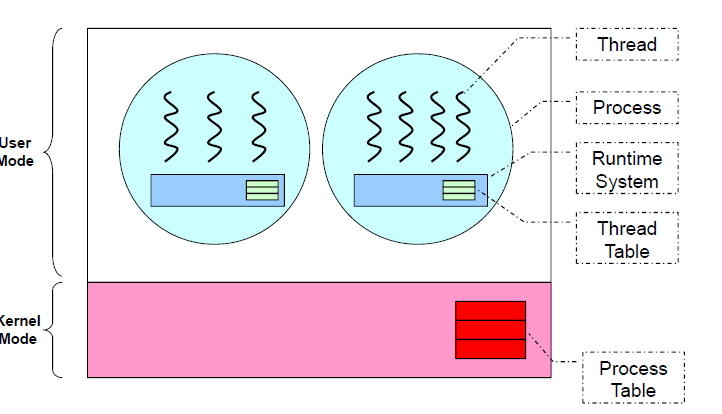
\includegraphics[width=0.25\textwidth]{4_1.png}
\end{figure}
The advantages of user thread model are
\begin{itemize}[itemsep=0pt]
  \item Can have multithreaded process on \textit{any} OS
  \item Thread operations are just library calls
  \item Generally more configurable and flexible, e.g. the scheduling algorithm can be customized.
\end{itemize}
However, the disadvantages are
\begin{itemize}[itemsep=0pt]
  \item OS is not aware of threads, therefore the scheduling of threads across processes is performed at process level. Therefore, one thread blocked will cause the process to be blocked, and therefore all other process will be blocked
  \item It cannot exploit multiple CPUs.
\end{itemize}
\end{definition}
\begin{definition}[Kernel Thread]
\normalfont Thread is implemented in the OS, and thread operation is handled as system calls.\\
This makes thread-level scheduling possible, and kernel may make use of threads for its own execution.
\begin{figure}[h]
\centering
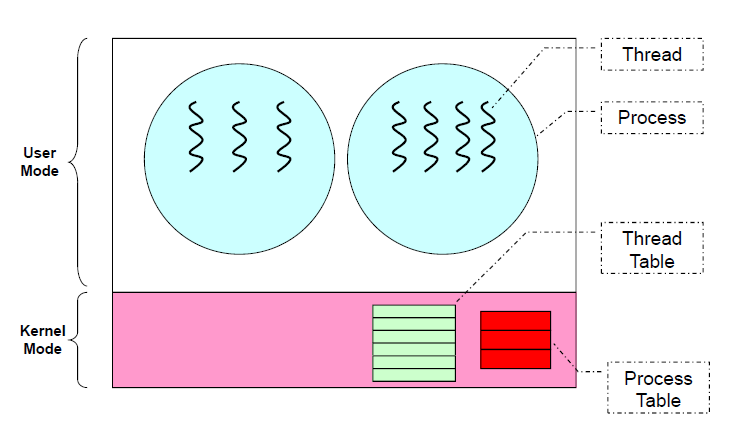
\includegraphics[width=0.25\textwidth]{4_2.png}
\end{figure}
The advantages of kernel thread model are
\begin{itemize}[itemsep=0pt]
  \item Kernel can schedule on thread levels, therefore more than 1 thread in the same process can run simultaneously on multiple CPUs.
\end{itemize}
However, the disadvantages are
\begin{itemize}[itemsep=0pt]
  \item Thread operations is now a system call, which is slower, and more resource intensive
  \item If implemented with many features, then it will be expensive and an overkill for simple program
  \item If implemented with few features, it is not flexible enough for some programs
\end{itemize}
\end{definition}
To take advantage of both models, in actual system, we use a hybrid thread model, where
\begin{itemize}[itemsep=0pt]
  \item there are both kernel and user threads
  \begin{itemize}[itemsep=0pt]
    \item OS schedule on kernel threads only
    \item User threads are binded to kernel threads
  \end{itemize}
\end{itemize}
\begin{figure}[h]
\centering
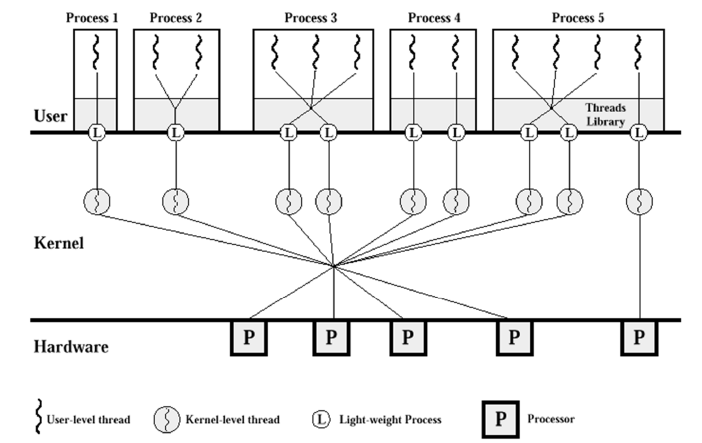
\includegraphics[width=0.25\textwidth]{4_3.png}
\end{figure}
This offers great flexibility, as we can limit the concurrency of any process/user.\\
Threads on a modern processor starts of a software mechanism and now become hardware native.
\subsection{POSIX Threads}
The thread in POSIX system can be used by including \texttt{\#include <pthread.h>}. The useful datatypes are
\begin{itemize}[itemsep=0pt]
  \item \texttt{pthread\_t}: data type to represent a thread id
  \item \texttt{pthread\_attr}: data type to represent attributes of a thread
\end{itemize}
Creation of a thread is done through
\texttt{pthread\_create(pthread\_t* tidCreated, const pthread\_attr\_t* threadAttributes, void* (*startRoutine) (void*), void* argForStartRoutine)}\\
This call returns $0$ for success and non-zero for errors.\\
Termination of a thread is done through
\texttt{int pthread\_exit(void* exitValue)}\\
Here, \texttt{exitValue} is the value to be returned to whoever synchronize with this thread. If it is not called, a pthread will terminate automatically at the end of startRountine, with no exit value returned.\\

Thread synchronizatin is done via
\texttt{int pthread\_join(pthread\_t threadID, void \*\*status)}\\
which waits for the termination of another pthread. It returns $0$ for success and nonzero for errors.
%\clearpage
\section{Inter-Process Communication(IPC)}
Since it is hard for cooperating process to share information, we need IPC mechanisms. There are two common IPC mechanisms, namely \textbf{shared memory} and \textbf{message passing}. There are two \textit{Unix-specific} IPC mechanisms, namely \textbf{pipe} and \textbf{signal}.
\subsection{Shared Memory}
Communication via \textbf{shared memory} is done via the following steps:
\begin{itemize}[itemsep=0pt]
  \item Process $P_1$ \underline{creates} a shared memory region $M$.
  \item Process $P_2$ \underline{attaches} memory region $M$ to its own memory space.
  \item $P_1$ and $P_2$ can now communicate using this memory region $M$.
\end{itemize}
The same model is also applicable to multiple processes haring same memory region.\\
The advantages of shared memory scheme are
\begin{itemize}[itemsep=0pt]
  \item \textbf{Efficient}, since only initial steps of creation and attachment involves PS
  \item \textbf{Easy to use}, since shared memory region behaves the same as normal memory space, so information of any size or type can be written easily.
\end{itemize}
The disadvantages are
\begin{itemize}[itemsep=0pt]
  \item \textbf{Synchronization}: Since it is shared resource, we need to have a proper way for synchronized access
  \item \textbf{Harder Implementation}.
\end{itemize}
For POSIX Shared Memory sheme, after the steps outlined above,
\begin{itemize}[itemsep=0pt]
  \item Detach $M$ from memory space after use
  \item Destory $M$. For this destory operation, only one process needs to do this, and it can only be done if $M$ is not attached to any process
\end{itemize}
\subsection{Message Passing}
Communication via \textbf{Message Passing} is done via the following steps:
\begin{itemize}[itemsep=0pt]
  \item Process $P_1$ prepares a message $M$ and send it to process $P_2$.
  \item Proecss $P_2$ receives the message $M$
  \item Message sending and receiving are usually provided as system calls
\end{itemize}
For this model, we need to concern about
\begin{itemize}[itemsep=0pt]
  \item \textbf{Naming}: how to identify the other party in the communication
  \item \textbf{Synchronization}: the behaviour of sending/receiving operations
\end{itemize}
Essentially, since OS is involved in message passing(sending and receiving), the message \textit{have to} be stored in kernel memory space.\\
There are two naming shemes:
\begin{definition}[Direct Communication]
\normalfont Sender/Receiver of the message explicitly name the other party. For example, \texttt{Send(P2, Msg); Receive(P1, Msg)}.\\
The characteristics of this scheme are
\begin{itemize}[itemsep=0pt]
  \item We need one link per pair of communicating processes
  \item We need to know the identity of the other party
\end{itemize}
\end{definition}
\begin{definition}[Indirect Communication]
\normalfont Message are sent to/received from message storage, usually known as \textbf{mailbox} or \textbf{port}. All messages are sent or retrieved from mailboxes.\\
The characteristics of this scheme is that one mailbox can be shared among a number of processes.
\end{definition}
There are also two synchronization behaviours:
\begin{definition}[Blocking Primitives(Synchronous)]
\normalfont 
\begin{itemize}[itemsep=0pt]
  \item \texttt{Send()} will cause sender to be blocked until the message is received.
  \item \texttt{Receive()} will cause receiver to be blocked until a message arrives.
\end{itemize}
\end{definition} 
\begin{definition}[Non-Blocking Primitives(Asynchronous)]
\normalfont 
\begin{itemize}[itemsep=0pt]
  \item \texttt{Send()} will have sender resume operation immediately.
  \item On \texttt{Receive()}, receiver either receive the message if available, or some indication that message is not ready yet.
\end{itemize}
\end{definition} 
The advantages of message passing is that
\begin{itemize}[itemsep=0pt]
  \item \textbf{Portable}: can easily be implemented on different processing environment
  \item \textbf{Easier Synchronization}: especially synchronous primitive is used, sender and receiver are implicitly synchronized.
\end{itemize}
The disadvantages are 
\begin{itemize}[itemsep=0pt]
  \item \textbf{Inefficient}, as it requires OS intervention
  \item \textbf{Harder to use}, as message are usually limited in size and/or format
\end{itemize}
\subsection{UNIX Pipes}
In Unix, a proces has 3 default comminucation channels:
\begin{itemize}[itemsep=0pt]
  \item stdin
  \item stderr
  \item stdout
\end{itemize}
Unix shell provides the ``$\mid$'' symbol to link the input/output channels of one process to another, and this is known as \textbf{piping}.\\
Essentially, a pipe can be shared between two processes, which makes the two processes to form a Producer-Consumer relationship.\\
The pipe behaves like an anonymous file, and access of this pipe is FIFO, i.e. access of data must be in order.\\

In implementation, pipe functions are implemented as \textbf{circular bounded byte buffer} with implicit synchronization:
\begin{itemize}[itemsep=0pt]
\item Writer will wait when buffer is full
\item Reader will wait when buffer is empty
\end{itemize} 
\textbf{Remark}: In variants of pipe, we can have multiple readers and writers. Also, the pipe can be either \textbf{half-duplex} or \textbf{full-duplex}.\\

The \texttt{C} system call is \texttt{int pipe(int fd[])}, where \texttt{fd[0]} is the reading end and \texttt{fd[1]} the writing end.\\

If we wan tto change the standard communication channels, we can use system calls named \texttt{dup()} and \texttt{dup2()}.
\subsection{Unix Signal}
Unix Signal is a form of inter-process communication, which serves as an asynchronous notification regarding an event sent to a process or a thread.\\
The recipient of the signal must handle the signal, by
\begin{itemize}[itemsep=0pt]
  \item A default set of handlers, or
  \item User supplied handler(only applicable to some signals)
\end{itemize}
The common signals in UNIX include kill, stop, continue, memory error, arithmetic error etc.
%\clearpage
\section{Synchronization}
The lack of synchronization will cause problem with \textbf{shared, modifiable resources} when concurrent processes access it in a interleaved fashion. This is known as \textbf{race condition}.\\
To resolve this, we need to implement a \textbf{critical section} where only one process can enter at any time. Correct Critical Section requires the following properties to be satisfied:
\begin{enumerate}
  \item \textbf{Mutual Exclusion}: If process $P_1$ is executing in critical section, all other processes are prevented from entering the critical section
  \item \textbf{Progress}: If no progress is in a critical section, one of the waiting processes should be granted access.
  \item \textbf{Bounded Wait}: After process $P_1$ request to enter critical section, there exists an upper bound of number of times other process can enter the critical section before $P_1$.
  \item \textbf{Independence}: Process \textit{not} executing in critical section should never block other process. 
\end{enumerate}
In case of incorrect synchronization, there will be problems like
\begin{enumerate}
  \item Deadlock, where all processes are blocked
  \item Livelock, where processes keep changing state to avoid deadlock and make no other progress
  \item Starvation, where some processes are blocked forever
\end{enumerate}
\subsection{Assembly Level Implementation}
We require an \textbf{atomic} instruction, named \texttt{TestAndSet}:
\[
\texttt{TestAndSet Register, MemoryLocation}
\]
The behaviour of the \texttt{TestAndSet} is to 
\begin{enumerate}
  \item Load the current content at \texttt{MemoryLocation} into \texttt{Register}
  \item Stores a $1$ into \texttt{MemoryLocation}
  \item Returns the Register's value to the user
\end{enumerate}
Therefore, \texttt{TestAndSet} will return $1$ if and only if the resource is used by another process.\\
With this observation, we can code \texttt{EnterCS} and \texttt{ExitCS} as follow:
\begin{verbatim}
void EnterCS(int* lock){
    while(TestAndSet(lock)==1);
}
void ExitCS(int* lock){
    *lock = 0;
}
\end{verbatim}
The implementation satisfies all four requirement of critical section, but the drawback is also evident: it employs a \textbf{busy waiting} scheme when waiting to enter CS, which is a wasteful use of processing power. We hope that such wait can essentially be turned into a blocked state of the process.
\subsection{High Level Language Implementation}
\begin{theorem}[Peterson's Algorithm]
\normalfont Suppose there are two processes $P_0$ and $P_1$. We will use 
\begin{enumerate}
  \item \texttt{Turn}, a variable that is set to indicate the turn belongs to the other process before checking for whether it is permitted to enter critical section
  \item \texttt{Want} array of 2 elements. This \texttt{Want} array allows process to indicate the intention of entering the critical section.
\end{enumerate}
Suppose process $0$ wants to enter critical section, it will set \texttt{Want[0]=1} and \texttt{Turn=1}, and check whether \texttt{Want[1]\&\&Turn==1} is true, which means that opponent wants and has the turn to use the critical section. If it is true, it will use a while loop to block $P_0$'s entrance.\\
After it successfully finishes critical section, \texttt{Want[0]=0}.
\end{theorem}
The assumption here is \textbf{writing to turn} is \textbf{atomic}.\\
The drawback of this algorithm is 
\begin{itemize}[itemsep=0pt]
  \item Buzy Waiting
  \item Low level
  \item Not general, as we may require more than mutual exclusion for synchronization
\end{itemize}
\subsection{High Level Synchronization Mechanism}
\begin{definition}[Semaphore]
\normalfont A semaphore is a generalized synchronization mechanism, which provides 
\begin{itemize}[itemsep=0pt]
  \item a way to block a number of processes, known as \textbf{sleeping process}, and 
  \item a way to unblock/wake up one, or more sleeping process
\end{itemize}
Semaphore will contain a integer valued number $S$. This $S$ can be initialized to any non-negative values initially.\\
Semaphore supports two \textbf{atomic} semaphore operations: \texttt{Wait(S)} and \texttt{Signal(S)}.
\begin{verbatim}
Wait(S)
    if(S<=0) blocks
    decrement S
Signal(S)
    increment S
    wake up one sleeping process if any
\end{verbatim}
The invariant of semaphore is
\[
S_\text{current} = S_\text{initial} + \#\text{signal}(S) - \#\text{wait}(S)
\]
where $\#\text{signal}(S)$ is number of signals operations executed, and $\#\text{wait}(S)$ is the number of wait operation \textbf{completed}.\\
With this invariance, we have $S_\text{current}+N_\text{CS}=1$ for binary semaphore. This ensures there is no deadlock.
\end{definition}
\subsection{Classical Synchronization Problems}
\subsubsection{Producer Consumer}
Suppose there is a shared bounded buffer of size $K$, where producer can produce item into the buffer if buffer is not full, and consumers can remove item from the buffer if buffer is not empty. There are multiple consumers and multiple producers.
\begin{figure}[h]
\centering
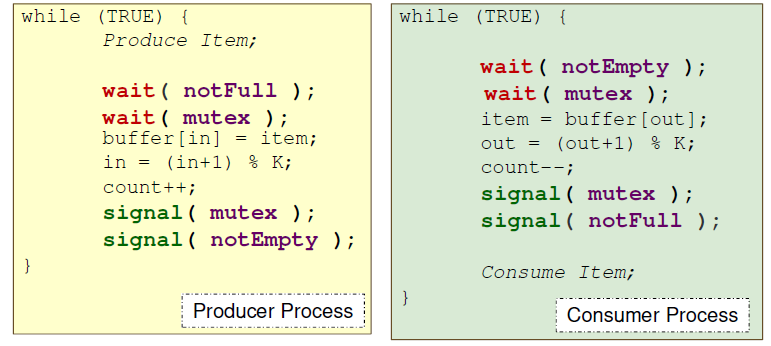
\includegraphics[width=0.5\textwidth]{5_1.png}
\end{figure}
is a blocking solution, if we initialize count, in , out to be $0$ and mutex has $S=1$, notFull has $S=K$ and notEmpty has $S=0$.
\subsubsection{Reader Writer}
Suppose there is a data structure $D$ where reader can retrieves information from $D$ and writer can modify information from $D$. Here we grant writer \textbf{exclusive access} to $D$, whereas multiple readers can access at the same time.
\begin{figure}[h]
\centering
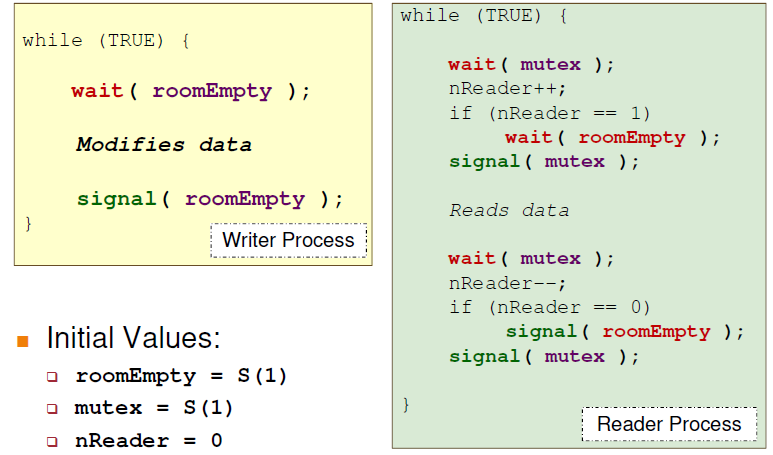
\includegraphics[width=0.5\textwidth]{5_2.png}
\end{figure}
is a solution that favours reader.
\subsubsection{Dining Philosophers}
There are 5 philosophers seating around the table, either thinking, hungry or eating. There is one chopstick to the left and another to the right of each philosopher, in total 5. We aim to let some of the philosopher to dine by successfully taking up 2 chopsticks that is on its left and right.\\
The code is detailed in the lecture notes.\\
An alternative is to use limited eater, where will use a semaphore with $S=4$ to limit number of seats to 4. and we use a semaphore on each chopsticks.
\end{document}